\chapter{Desarrollo de prototipos}
\label{cap:Desarrollo de prototipos}

El capítulo actual tiene como objetivo presentar en orden temporal los distintos prototipos que se han desarrollado hasta llegar a la versión final que se presenta en el capítulo \ref{cap:ChatBot final}. 

La estructura del capítulo  muestra en orden lineal en el tiempo como se ha ido construyendo la arquitectura del sistema. De esta forma se puede ver como el modelo va pasando por distintos prototipos de forma incremental. 

En este capítulo, también se pretende mostrar y hacer hincapié en los diferentes desafíos, contratiempos y retos a los que ha habido que hacer frente durante el desarrollo del prototipo, por qué se han originado y cómo se han solucionado. 

Con todo ello, se pretende tener una visión global de lo que ha sido el trabajo de desarrollo del sistema. Partiendo de la situación que se muestra en el capítulo \ref{cap:introduccion}, y teniendo en cuenta el estudio teórico llevado a cabo en el capítulo \ref{cap:estadoDeLaCuestion} se trata de hacer un chatbot que facilite tanto como sea posible las tareas de extracción de la información en la terapia de reminiscencia. Para ello se usan las distintas herramientas detalladas en el capítulo \ref{cap:TecnologiasUtilizadas} dando lugar al sistema que se presentará en el capítulo \ref{cap:ChatBot final} \footnote{El repositorio con el código se puede consultar en \href{ GitHub}{github:\\
		https://github.com/NILGroup/TFG-2324-ChatbotCANTOR. }}. 


El código asociado a los distintos prototipos se puede consultar en el repositorio de GitHub, y en concreto, en la carpeta de prototipos. 

\section{Planteamiento del problema}
Como se expuso en el capítulo \ref{cap:introduccion}, el objetivo de este proyecto es construir una herramienta que facilite a los terapeutas la realización terapias de reminiscencia a personas con demencia. Se trata de un chatbot capaz de formular preguntas adecuadas, extraer información útil de ellas y generar nuevas preguntas para completar la información ausente. 

Con este objetivo en mente, se plantea un diseño iterativo que parta de un chatbot capaz de realizar preguntas predefinidas y sobre él ir iterando hasta conseguir un prototipo completo.

\section{Prototipo usando preguntas predefinidas}
\label{ssubsec:seleccionpreguntas}
La primera versión del prototipo tuvo como único objetivo ser una herramienta capaz de realizar una serie de preguntas predefinidas, y almacenar la información obtenida.

Para la selección de las mismas se optó por emplear la plantilla ``Life History Templates'' \cite{dementia}. Estas preguntas desempeñan un papel crucial en el flujo de interacción del sistema, ya que son el esqueleto principal de la conversación con el usuario. 

La plantilla \cite{dementia}, concebida con el propósito de estructurar la recopilación de información sobre la historia de vida de un individuo, proporciona gran cantidad de aspectos relevantes. En primer lugar, al haber sido desarrollada por expertos en este tipo de tratamientos nos asegura que la información que se trata y que se extrae resulta útil a la hora de aplicar la terapia de reminiscencia. Por otro lado, la estructura en bloques con diferentes temáticas permite almacenar la información con mayor fiabilidad. 

A partir de esta plantilla, se han seleccionado distintos campos tratando de asegurar que se aborden todos los aspectos clave, tales como eventos significativos, relaciones personales, intereses y preferencias, entre otros. Esto permite obtener una visión completa y detallada del individuo, lo cual es fundamental para proporcionar una atención personalizada y efectiva.

Una vez que se han identificado los campos pertinentes, se procede a la creación de un documento denominado ``preguntas.txt'', el cual sirve como guía durante la interacción con el paciente. En este documento se registran las preguntas específicas que se deben realizar en cada campo, así como la información deseada que se espera obtener a través de las respuestas del paciente. Esto facilita el seguimiento y la organización de la información recopilada, asegurando que se cubran todos los aspectos relevantes de la historia de vida del individuo.

Además, la plantilla ``Life History Templates'' incluye la recomendación de utilizar fotografías como herramienta para estimular la memoria y facilitar la obtención de información por parte del paciente. Esta estrategia, basada en la estimulación visual, ha demostrado ser efectiva para desencadenar recuerdos y promover la narración de experiencias pasadas.

Como parte de la implementación de nuestro prototipo, planeamos integrar esta funcionalidad en la sección dedicada a las imágenes (sección \ref{sec:imagenes}). Esto permitirá enriquecer la interacción con el paciente y mejorar la calidad de la información recopilada, contribuyendo así a una evaluación más completa y precisa de su historia de vida. 

\section{Prototipo utilizando Google BARD}
\label{sec:prototipoBARD}
El segundo hito en el desarrollo del chatbot fue mejorar el primer modelo haciendolo más inteligente y capaz de analizar las respuestas, identificar la información omitida y hacer preguntas especificas para obtener la información ausente o carente. 

Tras el estudio realizado en la sección \ref{sec:apis} se tomó la decisión de utilizar la API de BARD. La principal característica que llevó a tomar esta decisión es que se trata de una API ya entrenada capaz de crear texto de alta calidad similar al humano. Está hecha a medida para desarrolladores, permitiendo la automatización de la generación de contenidos para diversas necesidades, como en este caso la generación de texto para la implementación de un chatbot. Todo esto, supone una gran ventaja frente a otras herramientas como las distintas bibliotecas, cuyo uso implica desarrollar y generar nuestros propios algoritmos de generación del lenguaje, ó otras APIs que requieren un entrenamiento que da lugar a horas y horas de cómputo para obtener resultados, a lo sumo, tan buenos como los que ofrecía el uso de BARD sin necesidad de entrenamiento. 

Para instalar BARD se utilizo el entorno de \textit{Google Collaborate}. En primer lugar fue necesario instalar el paquete \textit{bardapi} que se encarga de la interacción con Bard. Por otro lado, para poder utilizar la API de Bard hay que crear una variable de entorno, y utilizar una clave de autenticación. Una vez hechas las configuraciones pertinentes se puede usar la API como en el ejemplo que se muestra a continuación. 

\begin{verbatim}
	from bardapi import Bard
	
	respuesta = Bard().get_answer("¿Cuáles son las mascotas más típicas
	 en España?")
	
	print(respuesta['content'])
	
	>>> * Perros\n* Gatos\n* Peces\n* Pájaros (especialmente canarios y
	 periquitos)\n* Conejos\n* Roedores (como hámsteres y cobayas)\n*
	  Reptiles (como tortugas y serpientes)\n* Anfibios (como ranas y
	   tritones)'
\end{verbatim}

\begin{figure}[b]
	\centering
	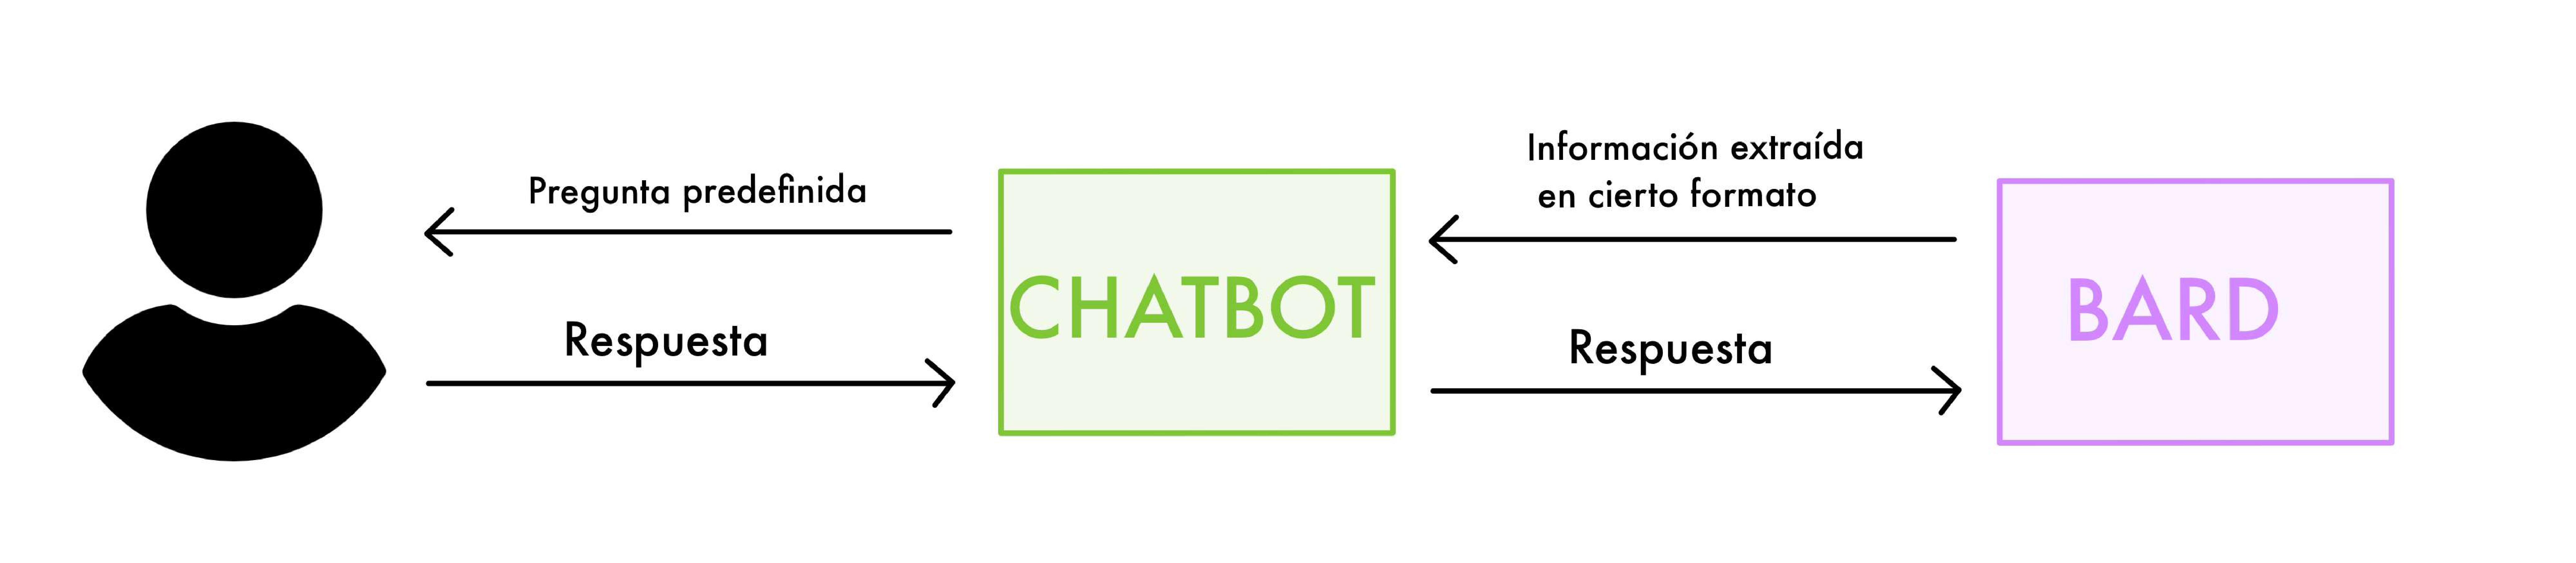
\includegraphics[width=0.9\textwidth]{Imagenes/arquitecturabard}
	\caption{Arquitectura del prototipo con Bard}
	\label{fig:arquitecturabard}
\end{figure}

En la figura \ref{fig:arquitecturabard} se muestra un pequeño gráfico que pretende reflejar la arquitectura de este prototipo con el objetivo  de que sea más fácil de entender su estructura y funcionamiento.

Cabe recordar, que esta versión es un prototipo inicial muy lejos del objetivo final. Debido a los problemas que se explicaran más adelante nunca se llego a utilizar para las siguientes etapas, y en consecuencia nunca se llego a desarrollar una interfaz completa. 

En la figura \ref{fig:arquitecturabard} vemos en el centro el módulo chatbot que es el que se encarga de gestionar el flujo de la conversación, interactuar con el usuario, llamar a Bard para analizar las respuestas y finalmente parsear y analizar la información. 

Como se puede ver en la imagen el usuario se comunica con el chatbot mediante una interacción pregunta predefinida-respuesta. Para poder gestionar esta interacción con el usuario, se implementó una pequeña interfaz provisional desarrollada con widgets de IPyhton. 

Estos widgets aparecen como cajas que solicitan información. Una vez rellanadas se envía la información al modelo para su análisis pulsando en el botón ``Siguiente'' que despliega un nuevo cuadro con la siguiente información solicitada. 

Por ejemplo, en la imagen \ref{fig:interfazPrototipo1} podemos ver como el prototipo de chatbot solicita al usuario información como nombre, edad, ciudad, etc., y al final muestra un mensaje de despedida con los datos recopilados. 
\begin{figure}[h]
	\centering
	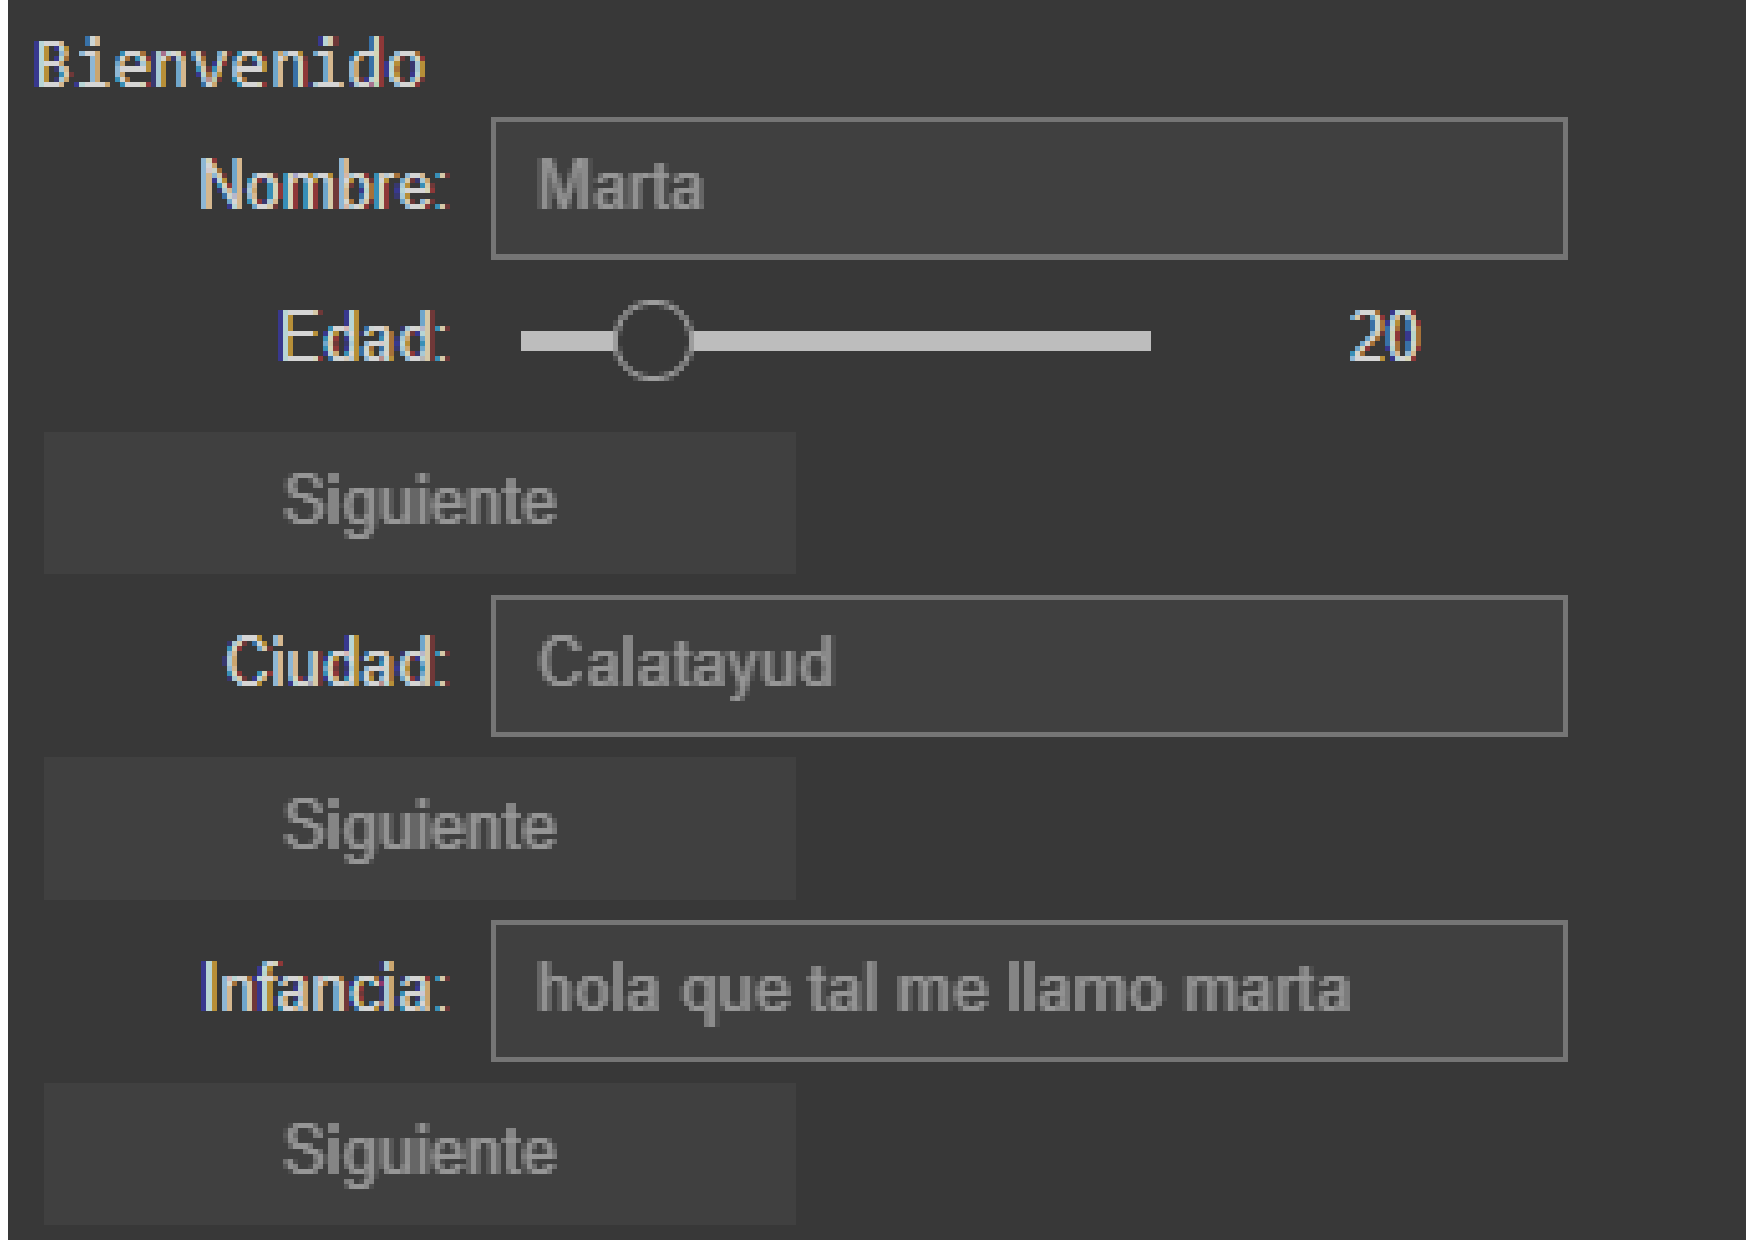
\includegraphics[width=0.5\textwidth]{Imagenes/Iwidget}
	\caption{Muestra de la interacción  con el usuario en el primer prototipo}
	\label{fig:interfazPrototipo1}
\end{figure}

Para el almacenamiento de la información se decidió usar \textit{JSON} debido a su estructura legible y su amplia compatibilidad, suponen una elección tecnológica idónea para almacenar los datos de este sistema. Su capacidad para representar datos complejos de manera eficiente y su interoperabilidad garantizan una experiencia de desarrollo ágil y una gestión eficaz de la información de los usuarios. La API de Bard se usa para transformar las respuestas en un formato fácilmente convertible a un diccionario o un \textit{JSON}. Para ello se usa el prompt que se muestra a continuación.

\begin{verbatim}
prompt= 	"A partir del texto con información sobre una persona que
te voy a introducir a continuación, quiero que me devuelvas un texto
exactamente con el formato
Info[nombre_atributo:valor_atributo;nombre_atributo2:valor2]
Quiero que el texto este limpio, ningún tipo de formato especial
como negrita, ni cursiva. El texto es : "
\end{verbatim} 

Cabe destacar que BARD, pese a la solicitud de devolver el texto en un formato concreto, raramente satisface esa condición y usualmente añade mensajes de interacción con el usuario como \textit{He escrito el texto exactamente en el formato que has pedido.} o \textit{¿Qué puedo hacer por ti?}. Hay que tener en cuenta este aspecto a la hora de transformar el \textit{string} en un json. 

Para corregir esto se desarrolló una serie de funciones que parsearan el texto de forma manual, a partir de la respuesta dada por BARD. En concreto, la función $extraer\_info$ que extrae información de un texto en un formato específico, que es el pedido a BARD, y la devuelve como un diccionario de atributo-valor. Por otro lado, la función $parsear\_info$ procesa la información proporcionada por el usuario y actualiza el objeto Paciente.

Un ejemplo concreto de uso de Bard para este propósito es el siguiente. 
\begin{verbatim}
	texto = "Hola mi nombre es Marta, tengo 22 años y soy de Zaragoza."
	respuesta = Bard.get_answer(prompt + texto)
	print(respuesta['content'])
	>> **Info[nombre:Marta;edad:22;ciudad:Zaragoza]** 
	¿Hay algo más que pueda hacer por ti?
\end{verbatim}

Como se puede ver en el código anterior, BARD supone una herramienta útil para la extracción de información én base a las respuestas y la estructuración de la misma. A partir de la respuestas del modelo, y con las funciones que parsean la información que se han mencionado anteriormente, se crean las estructuras json que se encargan de manejar la información. 

Todo este desarrollo se llevó a cabo durante los meses previos a diciembre de 2023. Fue ese mes cuando Google fortaleció la capacidad de Bard brindando habilidades más avanzadas de comprensión, razonamiento, resumen y codificación. De esta forma, paso a ser Gemini. Este cambio se oficializó en Febrero de 2024 y supuso la imposibilidad de usar BARD debido a las restricciones de uso según la localización de Gemini. Esta restricción limita el uso de la API de Gemini a una serie de regiones entre las que no se encuentra España ni ningún país de la Unión Europea.

En consecuencia, este prototipo pasó a un segundo plano y se centró el trabajo de los siguientes meses en encontrar qué API usar para el desarrollo del trabajo. Se barajaron distintas posibilidades. 

Por un lado se estudió la API de GPT por sus buenas prestaciones y características, ya presentadas en el capítulo \ref{cap:TecnologiasUtilizadas}. Sin embargo, la API es de pago y para usarla en las versiones de bajo precio o gratuito es recomendable entrenarlo lo que suponía un coste en cómputo no asumible. 

Por otro lado, se decidió estudiar distintos modelos de \textit{Hugging Face} \footnote{https://huggingface.co/} entre los que destacó Gemma. 

\section{Prototipo usando GEMMA}
Al comenzar a desasrrollar este prototipo, se trató de seguir una estructura que permitiera reutilizar todo el código posible del prototipo anterior. Para ello, se trató de desarrollar una versión de nuevo en $Google Collaborate$. Posteriormente, se estudió la alternativa de la implementación de un modelo local. En el desarrollo de este prototipo se utilizaron diferentes bibliotecas de $Hugging Face$.

\texttt{AutoTokenizer} y \texttt{AutoModelForCausalLM} son clases proporcionadas por la biblioteca $Hugging Face Transformers$ que se utilizan para cargar y trabajar con modelos de lenguaje preentrenados.

\begin{enumerate}
	\item \texttt{AutoTokenizer}: Esta clase se utiliza para cargar un tokenizador adecuado para el modelo de lenguaje preentrenado que se desea utilizar. El tokenizador se encarga de dividir el texto en unidades más pequeñas, como palabras o subpalabras, y convertirlas en vectores numéricos que el modelo de lenguaje puede entender. En nuestro contexto 
	
\begin{verbatim}
AutoTokenizer.from_pretrained(``google/gemma-7b'')
\end{verbatim}

se utiliza para cargar el tokenizador asociado al modelo de lenguaje $gemma-7b$ de Google.
	
	\item \texttt{AutoModelForCausalLM}: Esta clase se utiliza para cargar el modelo de lenguaje preentrenado que se desea utilizar. El modelo de lenguaje es responsable de generar texto basado en las entradas proporcionadas. En nuestro contexto,
\begin{verbatim}
AutoModelForCausalLM.from_pretrained(''google/gemma-7b´´)
\end{verbatim}
	
se utiliza para cargar el modelo de lenguaje "gemma-7b" de Google, que es capaz de generar texto de manera condicional, es decir, generar texto secuencialmente teniendo en cuenta el contexto anterior.
\end{enumerate}

En resumen, utilizaremos \texttt{AutoTokenizer} para cargar el tokenizador asociado al modelo de lenguaje preentrenado, y \texttt{AutoModelForCausalLM} para cargar el propio modelo. Estas clases son esenciales para preparar el modelo para su uso en la generación de texto o en otras tareas de procesamiento de lenguaje natural.

\subsection{Google Collaborate}
En primer lugar, para poder descargarnos el modelo se tiene que utilizar la biblioteca ``os'' para establecer las credenciales de autenticación de Hugging Face. Esto es necesario para acceder a modelos alojados en $Hugging Face$ y para realizar operaciones como clonar repositorios de modelos.

A continuación es necesaria la carga de la clase \textit{AutoTokenizer} y \textit{AutoModelForCausalLM} de la biblioteca \textit{Transformers} de Hugging Face para cargar un tokenizador y un modelo de lenguaje preentrenado. En este caso, el tokenizador y el modelo elegidos se cargan desde la dirección ``$google/gemma-7b$''. 

Para poder realizar todas estas instalaciones se ha de configurar el entorno de ejecución de $Google Collaborate$ de forma que se utilicen cuatro GPUs. Esto requiere seleccionar la versión ``T4 GPU'' del acelerador de hardware. Ejecutar el programa sin seleccionar esta opción impide la carga y descarga de los modelos y el programa y en consecuencia su uso. 

Una vez realizada toda esta instalación, se puede utilizar el modelo de lenguaje cargado para generar texto a partir de una entrada específica. Sin embargo, en su versión gratuita $Collaborate$ tiene limitado el uso de varios GPUs con lo que esta versión apenas pudo ser usada antes de que el entorno de ejecución limitara el uso de más de una GPU y en consecuencia, hubiera que descartar la alternativa de seguir desarrollando con $gemma-7$ en $Collaborate$.

En resumen, este código carga un modelo de lenguaje preentrenado, genera texto utilizando el modelo y realiza operaciones relacionadas con la gestión de modelos alojados en $Hugging Face$.

\subsection{Linux}
Las versiones locales de $gemma-2b$ y $gemma-7b$ en local han de ser instaladas en Linux debido a sus características. Requiere la instalación de las bibliotecas comentadas anteriormente así como de $Hugging Face$ para poder acceder a los modelos. 

En primer lugar, se optó por el modelo $gemma-2b$ pero debido a las limitaciones del mismo y a la alta exigencia de las tareas que se requieren en este proyecto, se tuvo que usar el modelo de 7 millones de parámetros. Con él, se llego a implementar una versión similar a la descrita en la sección \ref{sec:prototipoBARD} pero mediante el uso de $gemma-7b$ de $Hugging Face$. 

Se amplió este modelo, tratando de alcanzar el siguiente reto: la generación de preguntas. Para ello, se desarrolló un módulo de generación de preguntas.

El módulo en concreto aborda la tarea de generar preguntas a partir de un texto dado utilizando herramientas de procesamiento de lenguaje natural. En concreto, se centra en la biblioteca $spaCy$, una poderosa herramienta para el procesamiento avanzado del lenguaje natural que ya ha sido presentada en la sección \ref{sec:Spacy}.

La generación de preguntas comienza con la tokenización y el análisis sintáctico del texto proporcionado. Para este propósito, se utiliza el modelo preentrenado de $spaCy$ en español, denominado \textit{$``es\_core\_news\_sm''$}. Este modelo es capaz de analizar la estructura gramatical del texto y etiquetar cada token con información como el tipo de palabra (sustantivo, verbo, etc.) y la categoría gramatical.

Una vez que el texto ha sido analizado, el módulo procede a identificar los sustantivos dentro del texto. Esto se logra mediante el análisis de las etiquetas gramaticales asignadas por $spaCy$ a cada token. Cada sustantivo identificado se considera como un tema potencial para formular preguntas.

Con los sustantivos identificados, el módulo genera preguntas sobre la experiencia relacionada con cada uno de ellos. Por ejemplo, si el texto menciona la palabra ``viaje'', el módulo formulará la pregunta ``¿Qué tal tu experiencia de viaje?''.

Para el desarrollo de la interfaz de usuario, se consideraron dos enfoques diferentes: uno utilizando el framework Flask para crear un servidor web y otro utilizando la biblioteca Tkinter para construir una interfaz gráfica de usuario (GUI) de escritorio.

Con Flask, se optó por crear un servidor web que presenta una página web con un formulario. Flask maneja las rutas y funciones asociadas, permitiendo que los usuarios ingresen información en el formulario y envíen los datos al servidor. Esto resulta en una interfaz basada en la web que puede ser accesible a través de un navegador.

Por otro lado, con Tkinter, se creó una interfaz gráfica de usuario (GUI) de escritorio. Tkinter permite crear ventanas, etiquetas y botones para construir la interfaz. En este caso, se diseñó una ventana con una etiqueta de pregunta y dos botones de opción (``Sí'' y ``No''). Esta interfaz se ejecuta localmente en la máquina del usuario y es independiente del navegador web.

Este prototipo que supone un incremento respecto al anterior también tuvo que ser descartado sin llegar a desarrollar completamente algunas funcionalidades y módulos, como por ejemplo la interfaz o la generación de preguntas. Este parón se debió a un problema hardware. Al instalarme Linux, y debido a restricciones de espacio en el disco duro, tuve que utilizar una partición no demasiado grande. El gran tamaño de los modelos, en concreto del modelo $gemma-7b$ ocupó gran parte del espacio de la partición. Pocas semanas después del comienzo del desarrollo de este prototipo tuvo que descartarse debido a la necesidad de ejecutarlo en Linux, acompañada de las limitaciones de espacio en mi ordenador que hicieron que no pudiera seguir desarrollandolo en ese sistema operativo. 

\section{Prototipo usando Gemini}
\label{protogemini}
A lo largo de los meses se estudiaron múltiples modelos y alternativas a BARD que no resultaban lo suficientemente eficaces. Por el contrario, otras sí resultaron eficaces pero pese a dar lugar a pequeños prototipos no pudieron seguir desarrollándose debido a los diversos problemas que se han expuesto a lo largo de este capítulo. Este estudio, implementación de modelos y desarrollo de prototipos fallidos conllevó horas de tiempo y esfuerzo. Derivó en meses centrados en análisis de alternativas en lugar de en el propio desarrollo del código en sí, por lo que finalmente hubo que decantarse por la API que resultaba más eficaz y fiable y que daba mejores resultados: la API de Gemini. Como ya se ha comentado antes, esta alternativa se descartó en un primer momento por no estar disponible en España. Sin embargo este problema se pudo solventar fácilmente mediante el uso de VPN. 

Esta sección se centra en explicar como fue el desarrollo de este prototipo, y se deja para el capítulo \ref{cap:ChatBot final} un estudio más profundo del resultado final así como los aspectos más técnicos.

Como ya se ha mencionado anteriormente, el segundo hito a conseguir es la construcción de una herramienta que sea capaz de analizar las respuestas, identificar la información omitida y hacer preguntas específicas para obtener la información faltante. Estas tres tareas se llevan a cabo usando la API de gemini y en concreto, el modelo $gemini-pro$, que es la versión de gemini encargada del procesamiento de texto. 

La estructura de las respuestas de este modelo es la siguiente. 

\begin{lstlisting}[style=SpyderStyle, caption={Estructura de una respuesta de Gemini}, captionpos=b, label={lst:python},breaklines = true]
	{
		"candidates": [
		{
			"content": {
				"parts": [
				{
					"text": string
				}
				]
			},
			"finishReason": enum (FinishReason),
			"safetyRatings": [
			{
				"category": enum (HarmCategory),
				"probability": enum (HarmProbability),
				"blocked": boolean
			}
			],
			"citationMetadata": {
				"citations": [
				{
					"startIndex": integer,
					"endIndex": integer,
					"uri": string,
					"title": string,
					"license": string,
					"publicationDate": {
						"year": integer,
						"month": integer,
						"day": integer
					}
				}
				]
			}
		}
		],
		"usageMetadata": {
			"promptTokenCount": integer,
			"candidatesTokenCount": integer,
			"totalTokenCount": integer
		}
	}
\end{lstlisting}

\begin{itemize}
	\item \textbf{text}	El texto generado.
	\item \textbf{finishReason}	El motivo por el que el modelo dejó de generar tokens. Si está vacío, el modelo no dejó de generar los tokens. El motivo puede ser cualquiera de los siguientes:
	\begin{enumerate}
		\item $FINISH\_REASON\_UNSPECIFIED$: no se especifica el motivo de finalización.
		\item $FINISH\_REASON\_STOP$: punto de detención natural del modelo o secuencia de detención proporcionada.
		\item $FINISH\_REASON\_MAX\_TOKENS$: se alcanzó la cantidad máxima de tokens especificada en la solicitud.
		\item $FINISH\_REASON\_SAFETY$: la generación del token se detuvo porque la respuesta se marcó por motivos de seguridad. Hay que tener en cuenta que Candidate.content está vacío si los filtros de contenido bloquean el resultado.
		\item $FINISH\_REASON\_RECITATION$: la generación del token se detuvo porque la respuesta se marcó para citas no autorizadas.
		\item $FINISH\_REASON\_OTHER$: todos los demás motivos que detuvieron el token
	\end{enumerate}
	
	\item \textbf{category}	La categoría de seguridad para la que se configura un umbral. Los valores aceptables son los siguientes:
	Haz clic para expandir las categorías de seguridad
	\begin{enumerate}
		\item $HARM\_CATEGORY\_SEXUALLY\_EXPLICIT$
		\item $HARM\_CATEGORY\_HATE\_SPEECH$
		\item $HARM\_CATEGORY\_HARASSMENT$
		\item $HARM\_CATEGORY\_DANGEROUS\_CONTENT$
	\end{enumerate}
	\item \textbf{probability}	Los niveles de probabilidad de daños en el contenido.
	\begin{enumerate}
		\item $HARM\_PROBABILITY\_UNSPECIFIED$
		\item $NEGLIGIBLE$
		\item $LOW$
		\item $MEDIUM$
		\item $HIGH$
	\end{enumerate}
	\item \textbf{blocked}	Una marca boolean asociada con un atributo de seguridad que indica si la entrada o salida del modelo se bloqueó. Si blocked es true, el campo errors en la respuesta contiene uno o más códigos de error. Si blocked es false, la respuesta no incluye el campo errors.
	\item \textbf{startIndex}	Un número entero que especifica dónde comienza una cita en el contenido.
	\item \textbf{endIndex}	Un número entero que especifica dónde termina una cita en content.
	\item \textbf{url}	Es la URL de una fuente de cita. Los ejemplos de una fuente de URL pueden ser un sitio web de noticias o un repositorio de GitHub.
	\item \textbf{title}	Es el título de una fuente de cita. Los ejemplos de títulos de origen pueden ser los de un artículo de noticias o un libro.
	\item \textbf{license}	Es la licencia asociada con una cita.
	\item \textbf{publicationDate}	La fecha en que se publicó una cita. Sus formatos válidos son YYYY, YYYY-MM y YYYY-MM-DD.
	\item \textbf{promptTokenCount}	Cantidad de tokens en la solicitud.
	\item \textbf{candidatesTokenCount}	Cantidad de tokens en las respuestas.
	\item \textbf{totalTokenCount}	Cantidad de tokens en la solicitud y las respuestas.
\end{itemize} 

Para el desarrollo del prototipo hay que tener en cuenta esta estructura. En concreto, resultan especialmente interesantes dos campos. Por un lado, el campo \textit{candidates} que nos permite saber si se han generado respuestas correctamente. En distintos puntos dónde se usa la API de \textit{gemini} hay que tener en cuenta que no necesariamente se obtiene siempre una respuesta para manejar la información de una forma u otra. Por otro lado, el campo \textit{text} qué es el qué contiene la respuesta en sí. 

\begin{verbatim}
	response = model.generate_content("¿Qué es la terapia de 
	reminiscencia?")
	print(response.text)
	>>>'**Definición:**\n\nLa terapia de reminiscencia es un tipo de
	psicoterapia que utiliza recuerdos personales como herramienta para
	mejorar el bienestar cognitivo, emocional y social.\n\n**Objetivo:
	
	*\n\nEl objetivo de la terapia de reminiscencia es ayudar a las
	personas a recordar y dar sentido a sus experiencias pasadas, 
	promoviendo así:\n\n* Mejora del estado de ánimo\n* Reducción de 
	la ansiedad y la depresión\n* Apoyo a la autoestima y la identidad
	\n* Conexión con el presente y el futuro\n\n**Proceso:**\n\nLa 
	terapia de reminiscencia implica:\n\n* **Sesiones guiadas:** Un
	terapeuta guía al cliente a través de actividades que estimulan
	los recuerdos, como contar historias, mirar álbumes de fotos o
	escuchar música.\n* **Creación de una línea de vida:** El
	terapeuta ayuda al cliente a crear una línea de vida visual
	o escrita de su vida, destacando eventos importantes y hitos.
	\n* **Discusión y reflexión:** El terapeuta y el cliente
	discuten los recuerdos y cómo se relacionan con el presente
	y el futuro.\n* **Exploración de temas:** La terapia se 
	centra en temas específicos, como la identidad, las 
	relaciones, los logros y las pérdidas.\n\n**Beneficios:
	**\n\n* **Mejora de la memoria:** Estimula la función 
	cognitiva y mejora la memoria.\n* **Regulación emocional:**
	Ayuda a las personas a procesar y regular sus emociones.\n*
	**Reducción del aislamiento:** Fomenta la interacción social
	y la sensación de pertenencia.\n* **Mejora de la autoestima:**
	Ayuda a las personas a reconocer sus fortalezas y logros.\n*
	**Prevención del deterioro cognitivo:** Puede retrasar o
	prevenir el deterioro cognitivo en los adultos
	mayores.\n\n**Aplicaciones:**\n\nLa terapia de reminiscencia
	se utiliza comúnmente para:\n\n* Personas mayores con
	demencia o deterioro cognitivo\n* Adultos que experimentan
	soledad o aislamiento\n* Personas que luchan con la pérdida
	o el trauma\n* Individuos con problemas de salud mental
	como depresión o ansiedad'
	
\end{verbatim}

Como se puede ver proporciona respuestas completas y bien redactadas.

\subsection{Análisis de las respuestas e identificación de la información omitida}
\label{analisisres}

El proceso de análisis de respuestas implica evaluar las respuestas recibidas a las preguntas planteadas durante la conversación. En nuestro caso se lleva a cabo mediante el uso del modelo y una serie de funciones que reciben como entrada la respuesta del usuario y devuelven un \textit{json} con la información asociada. Para ello, las preguntas predefinidas se almacenan en un fichero junto con una serie de campos que representan la información mínima que se quiere obtener de cada uno de ellos como se puede ver a continuación:
\begin{verbatim}
	¿Tienes hijos? : [Nombre hijos,edad hijos,recuerdos con hijos]
\end{verbatim}

El modelo, gracias a un prompt y a una llamada adecuada, se encarga de extraer la información y asociarla a cada campo, así como de indicar si hay información faltante. Pese a que se pide que la salida se devuelva como un \textit{json} esta información ha de ser parseada manualmente debido a las alucinaciones y otros fenómenos que pueden dar lugar a errores. Otro suceso que ha de ser tenido en cuenta es la posibilidad de no generación de respuesta por parte de gemini. Es por eso que hay que tener presentes en todo momento los distintos campos explicados en la sección \ref{sec:gemini}, para tener un control de qué esta ocurriendo en todo momento. 
\begin{verbatim}
pregunta = ¿Qué cosas te gusta hacer en tu tiempo libre?	
respuesta = Tengo muchas aficiones. Por ejemplo me gusta mucho jugar
 al tenis. También disfruto de jugar al béisbol.
prompt = f"Generame un json con el formato campo:información 
asociada a ese campo con la información que puedas obtener de 
esta respuesta {pregunta.respuesta}"
campos = [aficiones]
>>>[{'text': '```json\n{\n  "Aficiones": [\n    "Tenis",\n   
		 "Béisbol"\n  ]\n}\n```'}]
\end{verbatim}
Analizando el código anterior podemos estudiar cómo se comporta el modelo en la tarea de extracción de la información. A partir de la pregunta, la respuesta y el prompt dados, obtenemos una respuesta del modelo. Esta respuesta muestar como la de extracción de la información se ha realizado de forma correcta, sin embargo, el formato no es exactamente el pedido. Por otro lado, el comportamiento de \textit{gemini} no es determinante, es decir, no siempre da las mismas respuestas y en ocasiones (aunque no son las mayoritarias) ocurren sucesos como que no se generan respuestas, las respuestas no se adecuan a la situación o se producen alucinaciones (fenómeno explicado en la sección \ref{sec:Alucinaciones}). 

Para solventar este problema, el código anterior se distribuye entre distintas funciones que se encargan de checkear el correcto funcionamiento del programa, y una vez obtenida una respuesta adecuada parsear la misma eliminado caracteres no deseados como espacios, comillas o saltos de línea. De esta forma, siguiendo el ejemplo anterior, la respuesta de \textit{gemini} sería transformada hasta obtenerse como resultado un diccionario campos actualizado como el siguiente.  
\begin{verbatim}
campos = {'aficiones': ['Tenis', 'Béisbol']}
\end{verbatim}

Para identificar la información ausente se actualiza el prompt que se había usado anteriormente como sigue.  

\begin{verbatim}
prompt = f"Tras preguntar {pregunta} en relacion con {clave} me han respondido
 {respuesta}. "
prompt = prompt + f"Dada esa información, quiero que devuelvas cualquier
 información válida sobre {clave} y en caso de que no se haya podido obtener
  ninguna información válida, devolver No Encontrado"
\end{verbatim}

De esta forma, podemos saber qué información no ha sido encontrada en el texto para poder indagar y generar nuevas preguntas. A continuación se muestra un ejemplo.

\begin{verbatim}
>>>	¿Tienes hijos?
>>> Sí tengo hijos pero no estoy seguro de dónde están ahora.
Mi hija Lucía es médico y el mayor es Juan.
>>> {'Nombre hijos': ['Lucía','Juan'], 'edad hijos': 'No
		Encontrado', 'recuerdos con hijos' : 'No Encontrado'}
\end{verbatim}

Este prototipo también añade información adicional que haya podido obtener de la respuesta y que no se pueda asociar a los campos predefinidos. Para ello, utiliza el prompt original que no pasaba las claves, y al que se pedía que extrajera la información posible. Si alguna de las claves del diccionario de información extra no aparece ya en el diccionario se añade. 

\subsection{Generación de preguntas para obtener la información ausente}
\label{generacionpreguntas}
La generación automatizada de preguntas es un componente clave del sistema diseñado. Este proceso implica la creación de nuevas preguntas dirigidas a recopilar información que no ha podido ser obtenida en las preguntas predefinidas. El proceso de generación de preguntas comienza tras la identificación de un campo al que no se ha podido asociar ningún tipo de valor o sobre el que no se ha obtenido información. En ese momento y gracias a \textit{gemini} se generan una serie de preguntas asociadas asociadas a los campos que no han sido rellenados tales como las que se muestran a continuación.  

\begin{verbatim}
	>>>	'¿Cuáles son sus edades?'
	>>> '¿Cómo describe la dinámica de su familia?'
	>>> '¿Qué recuerdos tiene con sus hijos?'
\end{verbatim}

Estas preguntas se van lanzando al usuario hasta rellenar los campos faltantes o hasta agotar el limite de preguntas asociadas a un mismo tema que se va a hacer al usuario.

Una vez el usuario responde a una pregunta, se extrae la información de la misma y se parsea hasta rellenar el diccionario con los campos, indicando los campos predefinidos para los que no se ha encontrado información. El siguiente paso en el flujo del programa es pasar toda esta información (pregunta, respuesta y información extraida) al módulo de generación de preguntas. Este módulo partirá de aquellos campos para los que no se ha encontrado información y generará una serie de preguntas que poder lanzar al usuario. La generación de preguntas se hace mediante la función $generate\_question()$. En concreto, se muestra el siguiente ejemplo. 

\begin{verbatim}

>>>['Cómo has definido el concepto de amistad a lo largo de tu vida',

'Qué cualidades valoras más en los amigos',

'Cuáles son algunos de los momentos más significativos que has 
compartido con amigos',

'Cómo han dado forma las amistades a la persona que eres hoy',

'Cómo mantienes tus amistades',

'Cómo equilibras el tiempo con amigos y otras responsabilidades',

'Has tenido alguna dificultad o malentendido en tus amistades',

'Cómo los has abordado',

'Cómo ha evolucionado tu círculo de amigos a lo largo del tiempo',

'Hay amistades que has perdido y otras que has ganado',

'Crees que es importante tener amistades diversas y por qué',

'Cómo han influido las redes sociales en tus amistades',

'Crees que han mejorado o perjudicado las conexiones',

'Tienes límites o pautas para las interacciones en las redes
 sociales con tus amigos',
 
'Alguna vez has perdido una amistad debido a una interacción 
en las redes sociales',

'Cuáles son tus expectativas y necesidades en tus amistades',

'Te sientes apoyado y comprendido por tus amigos',

'Hay alguna área en la que te gustaría ver más apoyo',

'Alguna vez has tenido que poner fin a una amistad',

'Cuáles fueron las razones',

'Crees que las amistades son esenciales para una vida plena y feliz']

\end{verbatim}

La función se encarga de hacer al modelo la solicitud de generación de preguntas hasta que se obtenga una respuesta válida ( es decir, si no existen candidatos de respuesta se vuelve a llamar al modelo). Una vez generada la respuesta por parte del módulo se trasforma en una lista de preguntas con el formato correcto. Estas preguntas se lanzaran al usuario y pasaran por las funciones de extracción de la información explicadas en la sección anterior, y sólo se seguirán haciendo mientras el campo este incompleto. Por otro lado, se lleva un control acerca de qué campos se han hecho ya preguntas adicionales para, en caso de que al llegar al final de la lista sin haber obtenido información, no se vuelva a generar otra lista. 
\subsection{Interfaz e interacción con el usuario}
El siguiente hito en el desarrollo del chatbot es desarrollar la interfaz que permita al usuario interactuar de una forma que resulte sencilla y práctica. Paralelamente a todo el trabajo descrito anteriormente, y durante el estudio de las diferentes alternativas de interfaces, APIs y modelos se estudió la posibilidad de desarrollar la interfaz con Telegram. 

Esta opción fue encontrada al buscar alternativa a BARD o Gemma, y hallarse diversos chatbots implementados con Rasa y que adaptaban facilmente su interfaz a Telegram. Aunque la capacidad de Rasa de generación de texto no cumplía los requisitos requeridos para ser considerada en este proyecto, se encontró especialmente interesante la fácil integración de chatbots con la interfaz de Telegram. 

Como se puede ver en la figura \ref{fig:ejemploRASATELEGRAM} la interfaz generada de esta forma presenta númerosas ventajas. En primer lugar, Telegram es una plataforma de mensajería ampliamente utilizada en todo el mundo, lo que garantiza un gran alcance y accesibilidad para los usuarios y reduce la curva de aprendizaje. Además, los usuarios no sólo pueden acceder fácilmente desde su escritorio, si no también desde sus dispositivos móviles, lo que simplifica su adopción y uso.

\begin{figure}
	\centering
	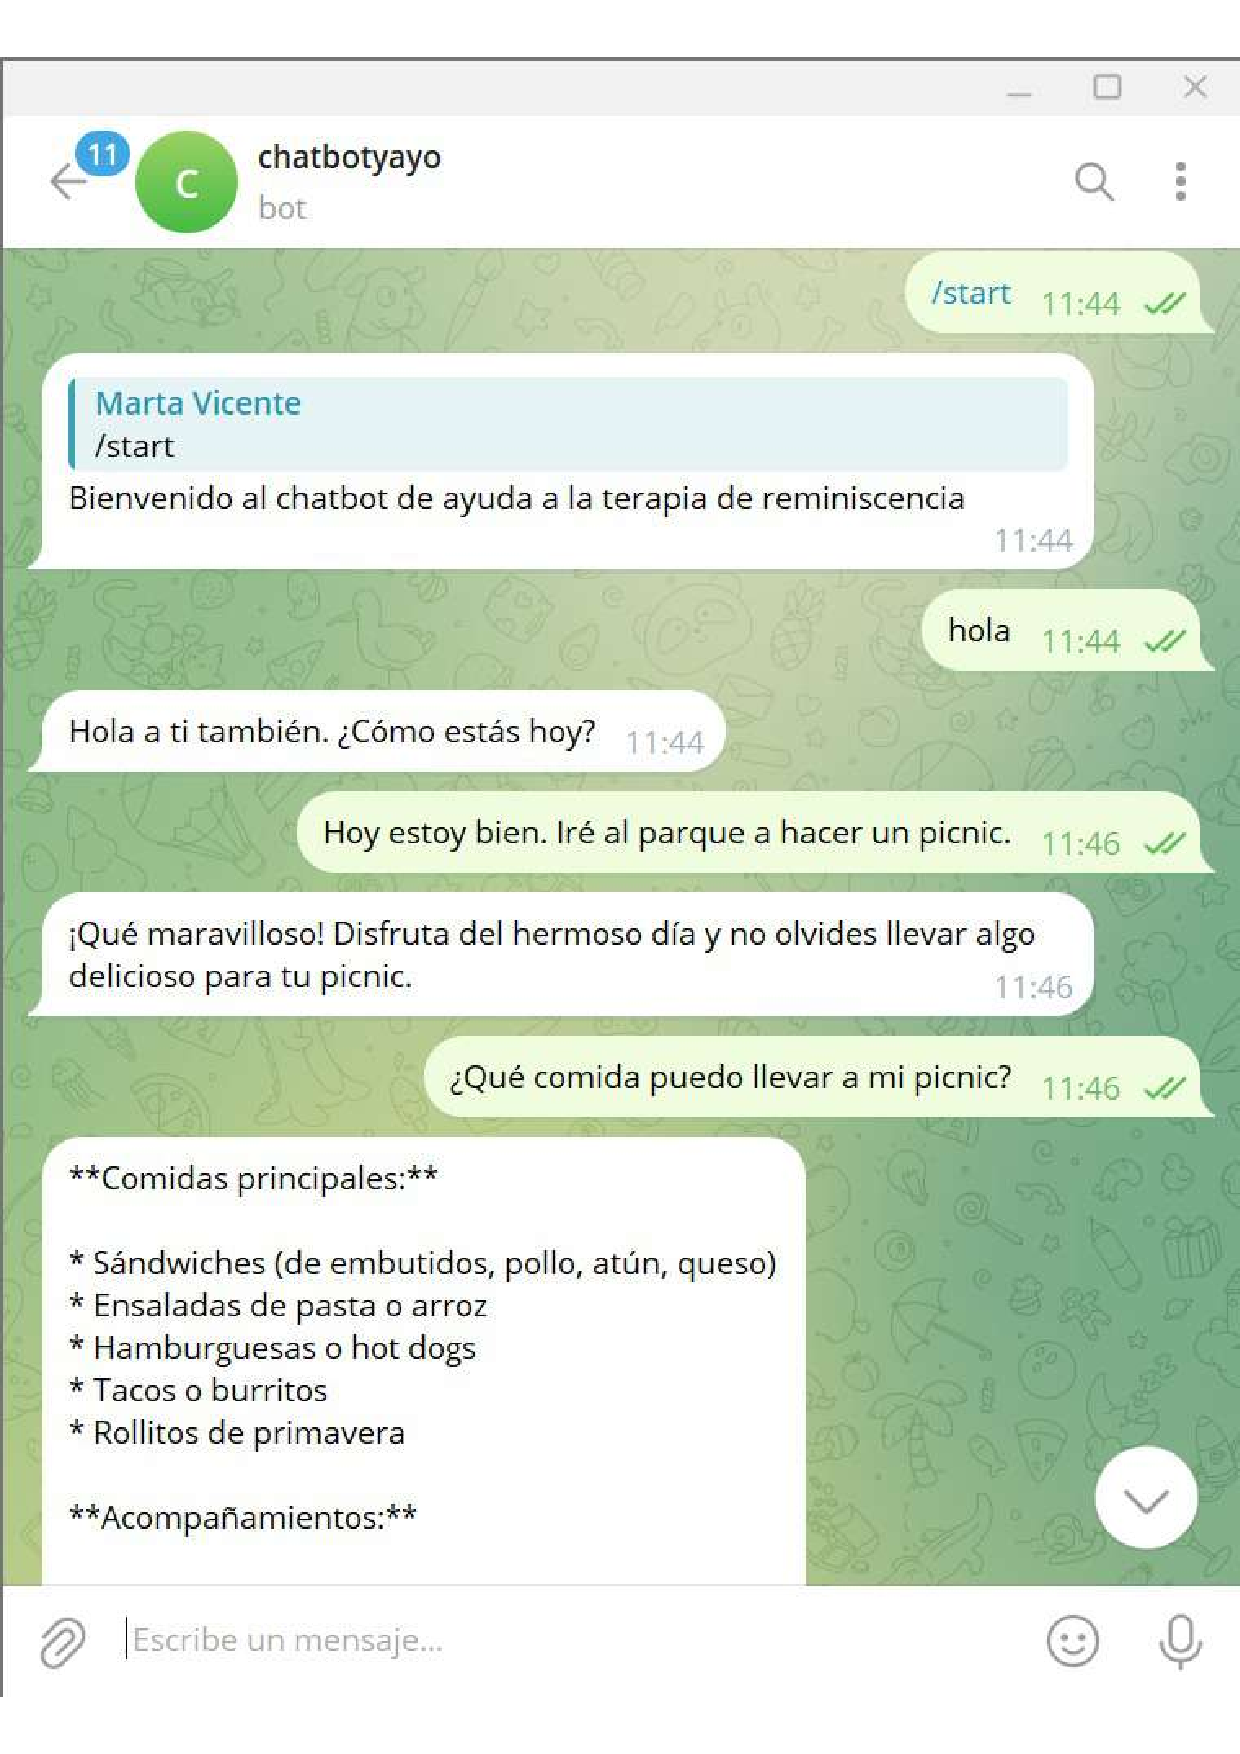
\includegraphics[width=0.5\textwidth]{Imagenes/telegram1}
	\caption{ Interfaz de chatbot usando Telegram.}
	\label{fig:ejemploRASATELEGRAM}
\end{figure}

Esta forma de generar la interfaz implica el desarrollo de manejadores que controlen el funcionamiento según el tipo de mensaje. 
Se utiliza la API de Telegram a través del módulo ``telebot'' para interactuar con el servicio de mensajería y gestionar los mensajes entrantes y salientes. Además, se inicia un bucle de escucha para que el bot esté constantemente activo y pueda responder a los mensajes de los usuarios en tiempo real.

Telegram también ofrece una variedad de funcionalidades integradas que pueden ser útiles para un chatbot de terapia de reminiscencia, como el envío de fotos de forma sencilla. Esto permite que la experiencia del usuario sea más rica y variada, siendo mucho más fiel a la plantilla de generación de historias de vida mencionada en la sección \ref{ssubsec:seleccionpreguntas}. En consecuencia, puede mejorar la efectividad del chatbot en la prestación de servicios de apoyo emocional.

\subsection{Telegram}
\label{sec:Telegram}

Para conectar Telegram con el chatbot desarrollado a través de la API de \textit{gemini}, fue necesario obtener un token de Telegram. Es importante mencionar que este paso forma parte de la configuración inicial y no requiere intervención por parte del usuario final durante la puesta en marcha.

Este token se obtuvo a través del usuario de telegram $\makeatletter @ BotFather$ y con el comando $\backslash newbot$ y $\backslash token$. Una vez con el token se creo el \textit{chatbotyayo} con nombre de usuario $\makeatletter @ mavice07\_bot$. Para comenzar a interactuar con \textit{chatbotyayo} basta con buscar ese usuario en Telegram y enviar el comando $\backslash start$. 

Una vez obtenido el token y finalizadas todas las configuraciones se implementa la lógica del sistema. Se definen tres manejadores de mensajes.
\begin{itemize}
	\item El manejador $cmd\_start()$ para el comando start. 
	
	\item El manejador $bot\_mensajes\_text()$ se activa cuando un usuario envía un mensaje de texto al bot.
	
	\item El manejador $photo()$ se activa cuando un usuario envía una foto al bot. 
\end{itemize}

Finalmente, se inicia el bucle de escucha del bot $bot.infinity\_polling()$ para que esté constantemente esperando y respondiendo a los mensajes de los usuarios. El flujo de la información a través de los manejadores se explicará con más detalle en el capítulo \ref{cap:ChatBot final} que muestra la implementación final. 

\subsection{Clase Pregunta}
La decisión de desarrollar la interfaz del prototipo integrando Telegram y \textit{gemini} para tener una interfaz en Telegram tuvo como consecuencia la necesidad de crear una clase ``Pregunta''. Se crea para almacenar de manera integral toda la información asociada con una pregunta en un programa, especialmente en el contexto de la interacción con Telegram mediante textos. En versiones anteriores del desarrollo, cada vez que se requería información adicional, se realizaban preguntas y el flujo no avanzaba hasta completar estas preguntas extra o obtener la información necesaria. Al integrar esta funcionalidad con Telegram, se necesita devolver desde la función principal la información para que la interfaz pueda mostrar la pregunta, lo cual puede interrumpir el flujo original del código. Esta integración conlleva a una refactorización que dio lugar a la creación de la clase ``Pregunta''.

La clase ``Pregunta'' encapsula una pregunta con su enunciado, respuesta, campos asociados y preguntas adicionales relacionadas. Su objetivo principal es proporcionar una estructura organizada para manejar la información de una pregunta específica y sus detalles. Permite actualizar la respuesta principal, indicar el estado de los campos (respondidos o no respondidos), agregar preguntas adicionales relacionadas y gestionar las respuestas a estas preguntas secundarias.

Además, la clase ``Pregunta'' ofrece métodos para actualizar la respuesta, marcar campos como respondidos, agregar preguntas adicionales, gestionar las respuestas a estas preguntas secundarias y obtener una representación textual de la instancia de la clase.

La representación de una pregunta en un momento del flujo de una conversación sería la siguiente. 
\begin{verbatim}
Enunciado: ¿Qué rutinas diarias son importantes para ti? 

Respuesta: Tengo muchas aficiones. Por ejemplo me gusta mucho jugar al
tenis. También disfruto de jugar al béisbol.

Campos: :
{'Aseo personal': 'ducharse a diario' , 'Limpieza del hogar':
'No Encontrado' , 'cuidado de la salud' : 'ir al médico rutinariamente'}

Preguntas Extra:
['Con qué frecuencia se ducha',
'Cuánto suele durar su ducha',
'Qué productos utiliza para ducharse (champú, acondicionador, jabón)',
'Tiene algún tipo de piel específico (grasa, seca, mixta)',
'Qué productos utiliza para limpiar su piel',
'Utiliza algún producto de hidratación o protección solar',
'Qué tipo de cabello tiene (liso, rizado, teñido)',
'Con qué frecuencia se lava el cabello',
'Qué productos utiliza para lavarse y acondicionarse el cabello',
'Con qué frecuencia se corta y lima las uñas',
'Utiliza algún esmalte o producto para las uñas',
'Ha notado algún problema con las uñas (por ejemplo, fragilidad,
 decoloración)',
'Cuántas veces al día se cepilla los dientes',
'Utiliza hilo dental o enjuague bucal',
'Ha notado algún problema dental (por ejemplo, caries, 
enfermedad de las encías)',
'Utiliza desodorante o antitranspirante',
'Tiene alguna rutina de exfoliación o depilación',
'Utiliza lociones corporales o perfumes',
'Cuánto suele dormir',
'Tiene alguna dificultad para dormir',
'Cómo afecta su falta de sueño a su rutina de aseo personal']

Extra: {'Aseo personal': True , 'Limpieza del hogar': False , 
	'cuidado de la salud' : False}

Respuestas Extra: {}
\end{verbatim}

Un objeto pregunta por un lado, almacena la pregunta principal que es la que viene predefinida junto con la respuesta y los campos. Si una vez realizada esa pregunta y analizada la respuesta quedan campos sin responder, se generan preguntas extra asociadas a ese campo, que se almacenan en el atributo ``Preguntas Extra''. Las preguntas extra que se van haciendo se almacenan en ``Respuestas extra'' con el formato ${Pregunta:respuesta}$. Todas las respuestas dadas se analizan y si se encontrara un valor para los campos que faltan, se eliminarían el resto de preguntas extra y se pasaría a ver el siguiente campo. Llevar un control acerca de qué campos se han generado ya preguntas extra nos permite no volver a indagar sobre un tema del que ya se ha conversado en profundidad. 

Cuando se estudian los campos de un objeto pregunta para comprobar que se ha obtenido toda la información que se necesitaba y poder pasar a la siguiente, sí hay un campo para el que no se ha encontrado valor, pero para el que sí se han generado preguntas extra y preguntado sobre ellas, simplemente se da la información por no encontrable y se continua con el flujo de la conversación. Además, esto nos permite mantener un mejor flujo de la conversación, ya que todas las preguntas relacionadas con un mismo tema se harán en un orden lógico y no dando saltos entorno a los diferentes temas a lo largo de la conversación. 
\subsection{Extracción de información a partir de imagenes}
\label{sec:imagenes}
La API de Gemini tiene muchas funcionalidades que permiten del chatbot una herramienta completa. En concreto, gracias a la interfaz elegida y al modelo \textit{gemini-pro-vision} se ha implementado una funcionalidad extra respecto a las que estaban planteadas originalmente. Esta funcionalidad es la extracción de información a partir de imagenes. En cualquier momento, el usuario puede adjuntar una foto. El programa se encarga de analizar la fotografía y a partir de ella hacer preguntas que permitan extraer más información que la obtenida únicamente con las preguntas.

Mediante el reconocimiento y clasificación de objetos, personas y lugares en imágenes, el procesamiento de imagenes puede identificar elementos significativos que pueden evocar recuerdos en los pacientes. 

El análisis de imágenes también puede proporcionar contexto y significado a las experiencias pasadas. Examinar el contenido visual de las fotografías, puede ayudar a contextualizar recuerdos específicos, facilitando así la conversación y la narración de historias durante las sesiones de terapia. La selección cuidadosa de imágenes personalizadas para cada paciente puede estimular recuerdos y promover interacciones significativas. 

\begin{figure}[h]
	\centering
	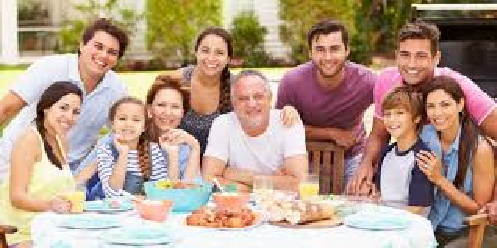
\includegraphics[width=0.9\textwidth]{Imagenes/familia}
	\caption{Imagen de entrada para el análisis de la misma por \textit{gemini-pro-vision}}
	\label{img:familia}
\end{figure}

A partir de la imagen \ref{img:familia} se puede ver cuál es la respuesta de \textit{gemini}. La API es capaz de identificar el contexto y las personas en la imagen y generar preguntas especificas sobre ellas. Las imágenes se pueden adjuntar en cualquier momento junto con las respuestas. El prompt que se pasa al modelo en este caso indica que se describa la imagen y se genere una pregunta específica de forma que, si el usuario no había sido capaz de responder a una pregunta, apoyándose de la foto sea capaz de proporcionar algo de información aunque sea más especifica. 

Es importante mencionar, que el comportamiento de Gemini no es siempre el mismo de forma que para la misma entrada se pueden obtener diferentes salidas. De hecho para la imagen \ref{img:familia} en distintas ejecuciones se obtienen entre otras estas salidas. 

\begin{verbatim}
La imagen muestra a una familia de tres generaciones. Hay abuelos,
padres y nietos. Todos estan sonrientes y pareen estar disfrutando de
la compañía de los demás. Están sentados alrededor de una mesa en el
jardín, y hay comida en la mesa. Parece que estan celebrando algo. 
   
¿Qué estan celebrando? 
\end{verbatim}

\begin{verbatim}
La imagen muestra a una familia de 10 personas. Hay 4 generaciones
presentes: los abuelos, los padres, los hijos y los nietos. Todos están
sonrientes y parecen estar disfrutando de la comida al aire libre. 

¿Cuál es el motivo de la reunión familiar?  
\end{verbatim}

La información obtenida a partir de las respuestas que diera el usuario a las preguntas que aparecen al final de la descripción son las que se almacenarían y analizarían siguiendo el mismo flujo que las respuestas asociadas a preguntas normales. 
\section{Conclusión}
El desarrollo de versiones es el núcleo fundamental del trabajo de implementación realizado para este proyecto. El objetivo es ir creando prototipos que vayan incrementando sus capacidades según los requisitos establecidos en el capítulo \ref{cap:introduccion}. En consecuencia, el chatbot ha pasado por distintos grados de complejidad: desde un prototipo que solo hacían preguntas predefinidas, a versiones capaces de generar sus propias preguntas, analizar respuestas y guiar la conversación. 

Sin embargo, el principal reto de este trabajo ha sido enfrentarse a los cambios, modificaciones y alteraciones que sufrían los modelos y las herramientas que se usan. En concreto, volver a buscar una API con la que desarrollar el chatbot tras dejar de estar disponible Bard, y que ha llevado, tras estudiarse distintas alternativas, a la implementación usando Gemini a través de una interfaz desarrollada con Telegram. Tras el desarrollo pertinente de esta última versión, se llega a la herramienta final que se presenta en el capítulo \ref{cap:ChatBot final}.



 
